% Created by tikzDevice version 0.10.1 on 2018-03-11 19:38:26
% !TEX encoding = UTF-8 Unicode
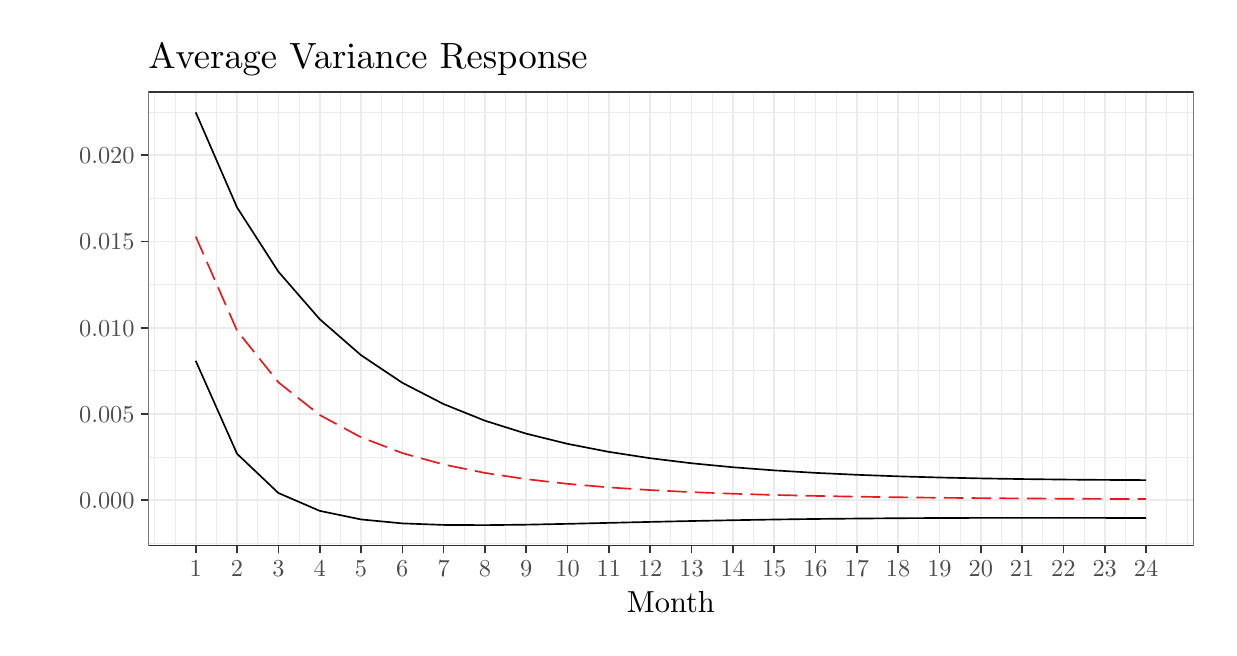
\begin{tikzpicture}[x=1pt,y=1pt]
\definecolor{fillColor}{RGB}{255,255,255}
\path[use as bounding box,fill=fillColor,fill opacity=0.00] (0,0) rectangle (426.79,216.81);
\begin{scope}
\path[clip] (  0.00,  0.00) rectangle (426.79,216.81);
\definecolor{drawColor}{RGB}{255,255,255}
\definecolor{fillColor}{RGB}{255,255,255}

\path[draw=drawColor,line width= 0.6pt,line join=round,line cap=round,fill=fillColor] (  0.00,  0.00) rectangle (426.79,216.81);
\end{scope}
\begin{scope}
\path[clip] ( 43.57, 29.59) rectangle (421.29,193.67);
\definecolor{fillColor}{RGB}{255,255,255}

\path[fill=fillColor] ( 43.57, 29.59) rectangle (421.29,193.67);
\definecolor{drawColor}{gray}{0.92}

\path[draw=drawColor,line width= 0.3pt,line join=round] ( 43.57, 30.48) --
	(421.29, 30.48);

\path[draw=drawColor,line width= 0.3pt,line join=round] ( 43.57, 61.64) --
	(421.29, 61.64);

\path[draw=drawColor,line width= 0.3pt,line join=round] ( 43.57, 92.79) --
	(421.29, 92.79);

\path[draw=drawColor,line width= 0.3pt,line join=round] ( 43.57,123.95) --
	(421.29,123.95);

\path[draw=drawColor,line width= 0.3pt,line join=round] ( 43.57,155.10) --
	(421.29,155.10);

\path[draw=drawColor,line width= 0.3pt,line join=round] ( 43.57,186.25) --
	(421.29,186.25);

\path[draw=drawColor,line width= 0.3pt,line join=round] ( 45.81, 29.59) --
	( 45.81,193.67);

\path[draw=drawColor,line width= 0.3pt,line join=round] ( 53.27, 29.59) --
	( 53.27,193.67);

\path[draw=drawColor,line width= 0.3pt,line join=round] ( 68.20, 29.59) --
	( 68.20,193.67);

\path[draw=drawColor,line width= 0.3pt,line join=round] ( 83.13, 29.59) --
	( 83.13,193.67);

\path[draw=drawColor,line width= 0.3pt,line join=round] ( 98.06, 29.59) --
	( 98.06,193.67);

\path[draw=drawColor,line width= 0.3pt,line join=round] (112.99, 29.59) --
	(112.99,193.67);

\path[draw=drawColor,line width= 0.3pt,line join=round] (127.92, 29.59) --
	(127.92,193.67);

\path[draw=drawColor,line width= 0.3pt,line join=round] (142.85, 29.59) --
	(142.85,193.67);

\path[draw=drawColor,line width= 0.3pt,line join=round] (157.78, 29.59) --
	(157.78,193.67);

\path[draw=drawColor,line width= 0.3pt,line join=round] (172.71, 29.59) --
	(172.71,193.67);

\path[draw=drawColor,line width= 0.3pt,line join=round] (187.64, 29.59) --
	(187.64,193.67);

\path[draw=drawColor,line width= 0.3pt,line join=round] (202.57, 29.59) --
	(202.57,193.67);

\path[draw=drawColor,line width= 0.3pt,line join=round] (217.50, 29.59) --
	(217.50,193.67);

\path[draw=drawColor,line width= 0.3pt,line join=round] (232.43, 29.59) --
	(232.43,193.67);

\path[draw=drawColor,line width= 0.3pt,line join=round] (247.36, 29.59) --
	(247.36,193.67);

\path[draw=drawColor,line width= 0.3pt,line join=round] (262.29, 29.59) --
	(262.29,193.67);

\path[draw=drawColor,line width= 0.3pt,line join=round] (277.22, 29.59) --
	(277.22,193.67);

\path[draw=drawColor,line width= 0.3pt,line join=round] (292.15, 29.59) --
	(292.15,193.67);

\path[draw=drawColor,line width= 0.3pt,line join=round] (307.08, 29.59) --
	(307.08,193.67);

\path[draw=drawColor,line width= 0.3pt,line join=round] (322.01, 29.59) --
	(322.01,193.67);

\path[draw=drawColor,line width= 0.3pt,line join=round] (336.94, 29.59) --
	(336.94,193.67);

\path[draw=drawColor,line width= 0.3pt,line join=round] (351.87, 29.59) --
	(351.87,193.67);

\path[draw=drawColor,line width= 0.3pt,line join=round] (366.80, 29.59) --
	(366.80,193.67);

\path[draw=drawColor,line width= 0.3pt,line join=round] (381.73, 29.59) --
	(381.73,193.67);

\path[draw=drawColor,line width= 0.3pt,line join=round] (396.66, 29.59) --
	(396.66,193.67);

\path[draw=drawColor,line width= 0.3pt,line join=round] (411.59, 29.59) --
	(411.59,193.67);

\path[draw=drawColor,line width= 0.3pt,line join=round] (419.05, 29.59) --
	(419.05,193.67);

\path[draw=drawColor,line width= 0.6pt,line join=round] ( 43.57, 46.06) --
	(421.29, 46.06);

\path[draw=drawColor,line width= 0.6pt,line join=round] ( 43.57, 77.21) --
	(421.29, 77.21);

\path[draw=drawColor,line width= 0.6pt,line join=round] ( 43.57,108.37) --
	(421.29,108.37);

\path[draw=drawColor,line width= 0.6pt,line join=round] ( 43.57,139.52) --
	(421.29,139.52);

\path[draw=drawColor,line width= 0.6pt,line join=round] ( 43.57,170.68) --
	(421.29,170.68);

\path[draw=drawColor,line width= 0.6pt,line join=round] ( 60.73, 29.59) --
	( 60.73,193.67);

\path[draw=drawColor,line width= 0.6pt,line join=round] ( 75.66, 29.59) --
	( 75.66,193.67);

\path[draw=drawColor,line width= 0.6pt,line join=round] ( 90.59, 29.59) --
	( 90.59,193.67);

\path[draw=drawColor,line width= 0.6pt,line join=round] (105.52, 29.59) --
	(105.52,193.67);

\path[draw=drawColor,line width= 0.6pt,line join=round] (120.45, 29.59) --
	(120.45,193.67);

\path[draw=drawColor,line width= 0.6pt,line join=round] (135.38, 29.59) --
	(135.38,193.67);

\path[draw=drawColor,line width= 0.6pt,line join=round] (150.31, 29.59) --
	(150.31,193.67);

\path[draw=drawColor,line width= 0.6pt,line join=round] (165.24, 29.59) --
	(165.24,193.67);

\path[draw=drawColor,line width= 0.6pt,line join=round] (180.17, 29.59) --
	(180.17,193.67);

\path[draw=drawColor,line width= 0.6pt,line join=round] (195.10, 29.59) --
	(195.10,193.67);

\path[draw=drawColor,line width= 0.6pt,line join=round] (210.03, 29.59) --
	(210.03,193.67);

\path[draw=drawColor,line width= 0.6pt,line join=round] (224.96, 29.59) --
	(224.96,193.67);

\path[draw=drawColor,line width= 0.6pt,line join=round] (239.89, 29.59) --
	(239.89,193.67);

\path[draw=drawColor,line width= 0.6pt,line join=round] (254.82, 29.59) --
	(254.82,193.67);

\path[draw=drawColor,line width= 0.6pt,line join=round] (269.75, 29.59) --
	(269.75,193.67);

\path[draw=drawColor,line width= 0.6pt,line join=round] (284.68, 29.59) --
	(284.68,193.67);

\path[draw=drawColor,line width= 0.6pt,line join=round] (299.61, 29.59) --
	(299.61,193.67);

\path[draw=drawColor,line width= 0.6pt,line join=round] (314.54, 29.59) --
	(314.54,193.67);

\path[draw=drawColor,line width= 0.6pt,line join=round] (329.47, 29.59) --
	(329.47,193.67);

\path[draw=drawColor,line width= 0.6pt,line join=round] (344.40, 29.59) --
	(344.40,193.67);

\path[draw=drawColor,line width= 0.6pt,line join=round] (359.33, 29.59) --
	(359.33,193.67);

\path[draw=drawColor,line width= 0.6pt,line join=round] (374.26, 29.59) --
	(374.26,193.67);

\path[draw=drawColor,line width= 0.6pt,line join=round] (389.19, 29.59) --
	(389.19,193.67);

\path[draw=drawColor,line width= 0.6pt,line join=round] (404.12, 29.59) --
	(404.12,193.67);
\definecolor{drawColor}{RGB}{228,26,28}

\path[draw=drawColor,line width= 0.6pt,dash pattern=on 7pt off 3pt ,line join=round] ( 60.73,141.31) --
	( 75.66,107.33) --
	( 90.59, 88.66) --
	(105.52, 76.85) --
	(120.45, 68.79) --
	(135.38, 63.09) --
	(150.31, 58.96) --
	(165.24, 55.92) --
	(180.17, 53.66) --
	(195.10, 51.97) --
	(210.03, 50.69) --
	(224.96, 49.72) --
	(239.89, 48.98) --
	(254.82, 48.40) --
	(269.75, 47.96) --
	(284.68, 47.61) --
	(299.61, 47.33) --
	(314.54, 47.12) --
	(329.47, 46.94) --
	(344.40, 46.81) --
	(359.33, 46.69) --
	(374.26, 46.60) --
	(389.19, 46.53) --
	(404.12, 46.47);
\definecolor{drawColor}{RGB}{0,0,0}

\path[draw=drawColor,line width= 0.6pt,line join=round] ( 60.73, 96.41) --
	( 75.66, 62.83) --
	( 90.59, 48.67) --
	(105.52, 42.21) --
	(120.45, 39.11) --
	(135.38, 37.68) --
	(150.31, 37.13) --
	(165.24, 37.05) --
	(180.17, 37.22) --
	(195.10, 37.52) --
	(210.03, 37.87) --
	(224.96, 38.22) --
	(239.89, 38.54) --
	(254.82, 38.83) --
	(269.75, 39.08) --
	(284.68, 39.28) --
	(299.61, 39.43) --
	(314.54, 39.55) --
	(329.47, 39.63) --
	(344.40, 39.67) --
	(359.33, 39.69) --
	(374.26, 39.69) --
	(389.19, 39.66) --
	(404.12, 39.62);

\path[draw=drawColor,line width= 0.6pt,line join=round] ( 60.73,186.22) --
	( 75.66,151.84) --
	( 90.59,128.65) --
	(105.52,111.48) --
	(120.45, 98.47) --
	(135.38, 88.49) --
	(150.31, 80.79) --
	(165.24, 74.79) --
	(180.17, 70.10) --
	(195.10, 66.42) --
	(210.03, 63.52) --
	(224.96, 61.23) --
	(239.89, 59.41) --
	(254.82, 57.97) --
	(269.75, 56.84) --
	(284.68, 55.94) --
	(299.61, 55.24) --
	(314.54, 54.69) --
	(329.47, 54.26) --
	(344.40, 53.94) --
	(359.33, 53.70) --
	(374.26, 53.52) --
	(389.19, 53.40) --
	(404.12, 53.32);
\definecolor{drawColor}{gray}{0.20}

\path[draw=drawColor,line width= 0.6pt,line join=round,line cap=round] ( 43.57, 29.59) rectangle (421.29,193.67);
\end{scope}
\begin{scope}
\path[clip] (  0.00,  0.00) rectangle (426.79,216.81);
\definecolor{drawColor}{gray}{0.30}

\node[text=drawColor,anchor=base east,inner sep=0pt, outer sep=0pt, scale=  0.88] at ( 38.62, 43.03) {0.000};

\node[text=drawColor,anchor=base east,inner sep=0pt, outer sep=0pt, scale=  0.88] at ( 38.62, 74.18) {0.005};

\node[text=drawColor,anchor=base east,inner sep=0pt, outer sep=0pt, scale=  0.88] at ( 38.62,105.34) {0.010};

\node[text=drawColor,anchor=base east,inner sep=0pt, outer sep=0pt, scale=  0.88] at ( 38.62,136.49) {0.015};

\node[text=drawColor,anchor=base east,inner sep=0pt, outer sep=0pt, scale=  0.88] at ( 38.62,167.64) {0.020};
\end{scope}
\begin{scope}
\path[clip] (  0.00,  0.00) rectangle (426.79,216.81);
\definecolor{drawColor}{gray}{0.20}

\path[draw=drawColor,line width= 0.6pt,line join=round] ( 40.82, 46.06) --
	( 43.57, 46.06);

\path[draw=drawColor,line width= 0.6pt,line join=round] ( 40.82, 77.21) --
	( 43.57, 77.21);

\path[draw=drawColor,line width= 0.6pt,line join=round] ( 40.82,108.37) --
	( 43.57,108.37);

\path[draw=drawColor,line width= 0.6pt,line join=round] ( 40.82,139.52) --
	( 43.57,139.52);

\path[draw=drawColor,line width= 0.6pt,line join=round] ( 40.82,170.68) --
	( 43.57,170.68);
\end{scope}
\begin{scope}
\path[clip] (  0.00,  0.00) rectangle (426.79,216.81);
\definecolor{drawColor}{gray}{0.20}

\path[draw=drawColor,line width= 0.6pt,line join=round] ( 60.73, 26.84) --
	( 60.73, 29.59);

\path[draw=drawColor,line width= 0.6pt,line join=round] ( 75.66, 26.84) --
	( 75.66, 29.59);

\path[draw=drawColor,line width= 0.6pt,line join=round] ( 90.59, 26.84) --
	( 90.59, 29.59);

\path[draw=drawColor,line width= 0.6pt,line join=round] (105.52, 26.84) --
	(105.52, 29.59);

\path[draw=drawColor,line width= 0.6pt,line join=round] (120.45, 26.84) --
	(120.45, 29.59);

\path[draw=drawColor,line width= 0.6pt,line join=round] (135.38, 26.84) --
	(135.38, 29.59);

\path[draw=drawColor,line width= 0.6pt,line join=round] (150.31, 26.84) --
	(150.31, 29.59);

\path[draw=drawColor,line width= 0.6pt,line join=round] (165.24, 26.84) --
	(165.24, 29.59);

\path[draw=drawColor,line width= 0.6pt,line join=round] (180.17, 26.84) --
	(180.17, 29.59);

\path[draw=drawColor,line width= 0.6pt,line join=round] (195.10, 26.84) --
	(195.10, 29.59);

\path[draw=drawColor,line width= 0.6pt,line join=round] (210.03, 26.84) --
	(210.03, 29.59);

\path[draw=drawColor,line width= 0.6pt,line join=round] (224.96, 26.84) --
	(224.96, 29.59);

\path[draw=drawColor,line width= 0.6pt,line join=round] (239.89, 26.84) --
	(239.89, 29.59);

\path[draw=drawColor,line width= 0.6pt,line join=round] (254.82, 26.84) --
	(254.82, 29.59);

\path[draw=drawColor,line width= 0.6pt,line join=round] (269.75, 26.84) --
	(269.75, 29.59);

\path[draw=drawColor,line width= 0.6pt,line join=round] (284.68, 26.84) --
	(284.68, 29.59);

\path[draw=drawColor,line width= 0.6pt,line join=round] (299.61, 26.84) --
	(299.61, 29.59);

\path[draw=drawColor,line width= 0.6pt,line join=round] (314.54, 26.84) --
	(314.54, 29.59);

\path[draw=drawColor,line width= 0.6pt,line join=round] (329.47, 26.84) --
	(329.47, 29.59);

\path[draw=drawColor,line width= 0.6pt,line join=round] (344.40, 26.84) --
	(344.40, 29.59);

\path[draw=drawColor,line width= 0.6pt,line join=round] (359.33, 26.84) --
	(359.33, 29.59);

\path[draw=drawColor,line width= 0.6pt,line join=round] (374.26, 26.84) --
	(374.26, 29.59);

\path[draw=drawColor,line width= 0.6pt,line join=round] (389.19, 26.84) --
	(389.19, 29.59);

\path[draw=drawColor,line width= 0.6pt,line join=round] (404.12, 26.84) --
	(404.12, 29.59);
\end{scope}
\begin{scope}
\path[clip] (  0.00,  0.00) rectangle (426.79,216.81);
\definecolor{drawColor}{gray}{0.30}

\node[text=drawColor,anchor=base,inner sep=0pt, outer sep=0pt, scale=  0.88] at ( 60.73, 18.58) {1};

\node[text=drawColor,anchor=base,inner sep=0pt, outer sep=0pt, scale=  0.88] at ( 75.66, 18.58) {2};

\node[text=drawColor,anchor=base,inner sep=0pt, outer sep=0pt, scale=  0.88] at ( 90.59, 18.58) {3};

\node[text=drawColor,anchor=base,inner sep=0pt, outer sep=0pt, scale=  0.88] at (105.52, 18.58) {4};

\node[text=drawColor,anchor=base,inner sep=0pt, outer sep=0pt, scale=  0.88] at (120.45, 18.58) {5};

\node[text=drawColor,anchor=base,inner sep=0pt, outer sep=0pt, scale=  0.88] at (135.38, 18.58) {6};

\node[text=drawColor,anchor=base,inner sep=0pt, outer sep=0pt, scale=  0.88] at (150.31, 18.58) {7};

\node[text=drawColor,anchor=base,inner sep=0pt, outer sep=0pt, scale=  0.88] at (165.24, 18.58) {8};

\node[text=drawColor,anchor=base,inner sep=0pt, outer sep=0pt, scale=  0.88] at (180.17, 18.58) {9};

\node[text=drawColor,anchor=base,inner sep=0pt, outer sep=0pt, scale=  0.88] at (195.10, 18.58) {10};

\node[text=drawColor,anchor=base,inner sep=0pt, outer sep=0pt, scale=  0.88] at (210.03, 18.58) {11};

\node[text=drawColor,anchor=base,inner sep=0pt, outer sep=0pt, scale=  0.88] at (224.96, 18.58) {12};

\node[text=drawColor,anchor=base,inner sep=0pt, outer sep=0pt, scale=  0.88] at (239.89, 18.58) {13};

\node[text=drawColor,anchor=base,inner sep=0pt, outer sep=0pt, scale=  0.88] at (254.82, 18.58) {14};

\node[text=drawColor,anchor=base,inner sep=0pt, outer sep=0pt, scale=  0.88] at (269.75, 18.58) {15};

\node[text=drawColor,anchor=base,inner sep=0pt, outer sep=0pt, scale=  0.88] at (284.68, 18.58) {16};

\node[text=drawColor,anchor=base,inner sep=0pt, outer sep=0pt, scale=  0.88] at (299.61, 18.58) {17};

\node[text=drawColor,anchor=base,inner sep=0pt, outer sep=0pt, scale=  0.88] at (314.54, 18.58) {18};

\node[text=drawColor,anchor=base,inner sep=0pt, outer sep=0pt, scale=  0.88] at (329.47, 18.58) {19};

\node[text=drawColor,anchor=base,inner sep=0pt, outer sep=0pt, scale=  0.88] at (344.40, 18.58) {20};

\node[text=drawColor,anchor=base,inner sep=0pt, outer sep=0pt, scale=  0.88] at (359.33, 18.58) {21};

\node[text=drawColor,anchor=base,inner sep=0pt, outer sep=0pt, scale=  0.88] at (374.26, 18.58) {22};

\node[text=drawColor,anchor=base,inner sep=0pt, outer sep=0pt, scale=  0.88] at (389.19, 18.58) {23};

\node[text=drawColor,anchor=base,inner sep=0pt, outer sep=0pt, scale=  0.88] at (404.12, 18.58) {24};
\end{scope}
\begin{scope}
\path[clip] (  0.00,  0.00) rectangle (426.79,216.81);
\definecolor{drawColor}{RGB}{0,0,0}

\node[text=drawColor,anchor=base,inner sep=0pt, outer sep=0pt, scale=  1.10] at (232.43,  5.50) {Month};
\end{scope}
\begin{scope}
\path[clip] (  0.00,  0.00) rectangle (426.79,216.81);
\definecolor{drawColor}{RGB}{0,0,0}

\node[text=drawColor,anchor=base west,inner sep=0pt, outer sep=0pt, scale=  1.32] at ( 43.57,202.22) {Average Variance Response};
\end{scope}
\end{tikzpicture}
